\section{Combining Learning and Control}
\label{sec:framework}

%Overview. Learning background.  Control background.
\SYSTEM{} combines learning with control to tackle both complexity and
dynamics.  \figref{fig:overview} shows a detailed overview of
\SYSTEM{}.  A mobile system runs an application and some small number
of measurements are taken and sent to a server. The server uses a
hierarchical Bayesian model to combine these measurements with ones
taken on other devices and with measurements of other applications.
Using this large volume of data, the HBM produces an
application-specific model of performance and power for all resource
configurations.  The model is sent to a lightweight control system
(LCS) that manages the device, adjusting resource usage to meet
application performance requirements with minimal energy.  The learned
models are stored a performance hash table (PHT), which is the
interface between the remote HBM and the LCS that manages the device.
The expensive process of constructing the PHT is done by the server.
Once built, the PHT allows the LCS to apply the learned models in
constant ($O(1)$) time.  This section provides a brief overview of the
relevant learning and control techniques used in \SYSTEM{}, and then
describes the interface that combines them.

\subsection{The Hierarchical Bayesian Model}
\label{sec:framework:HBM}

%\PUNT{

Machine learning models are predictive in nature.  Given some
observations of a system, they create a model to predict future
behavior in unobserved settings. \SYSTEM{} uses a hierarchical
Bayesian model (HBM), based on LEO \cite{LEO}, to turn observations of
applications' performance and power given some resource allocation
into predictions about how other, unobserved resource allocations will
alter that performance and power.  The HBM provides a statistically
sound framework for learning across applications and devices.

The HBM is non-parametric in terms of resource configurations. Instead
of modeling performance of a configuration as a function of exact
number of cores or clockspeed, it captures correlations between
configurations.  Hence, the HBM is well suited to learning complicated
configuration spaces, like those in
\figsref{fig:lavamd_contour}{fig:kmeans_contour}.  The non-smoothness
and application-specificity of these configuration spaces means that
parametric models -- based on clockspeed/cores -- will not perform
well.  In contrast, the HBM requires fewer assumptions about the
relationship between configurations and performance/power and is thus
more robust for this modeling problem \cite{LEO}.

\figrref{fig:online}{fig:HBM} compare \SYSTEM{} to \emph{online} and
\emph{offline} learning models.  The online model only uses
observations of the current application and it must be parametric in
the configuration space, since it has no other information. The online
model is thus highly dependent on the model parameterization; \eg{} if
the model is specified to be linear in frequency, but an application
is memory-bound, the online model will over-allocate resources.  The
offline model only uses information from previously observed
applications and lacks knowledge of the current application.  This
general model will capture trends -- \eg{} when most applications
should transition from LITTLE to big cores -- but it will miss key
inflection points for applications that deviate from the general
trend.

\begin{figure}

  \subfloat[]
  {
    %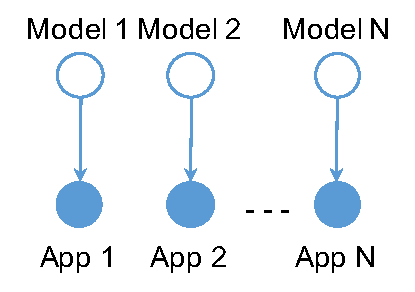
\includegraphics[width=.33\textwidth]{figures/Online.pdf}
    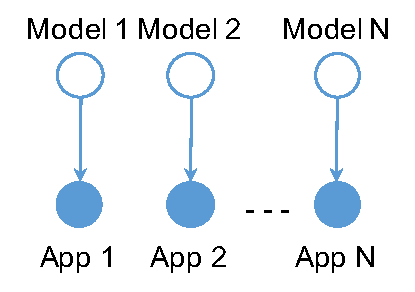
\includegraphics[width=.33\columnwidth]{figures/Online.pdf}

    \label{fig:online}
  }
  \subfloat[]
  {
    %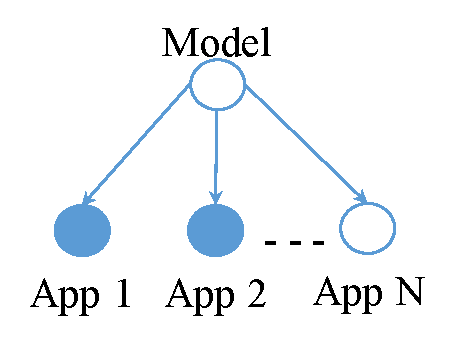
\includegraphics[width=.33\textwidth]{figures/Offline.pdf}
    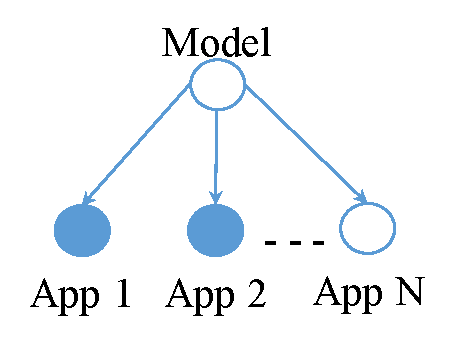
\includegraphics[width=.33\columnwidth]{figures/Offline.pdf}

    \label{fig:offline}
  }
  \subfloat[]
  {
    %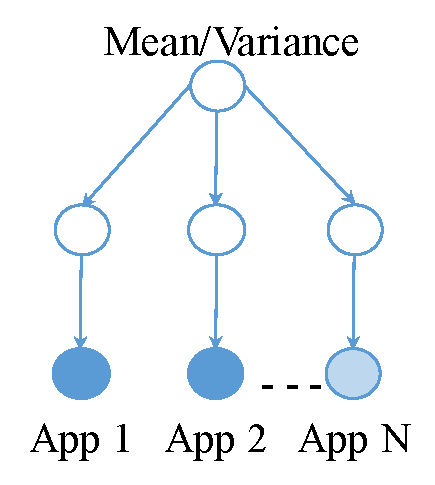
\includegraphics[width=.33\textwidth]{figures/HBM.pdf}
    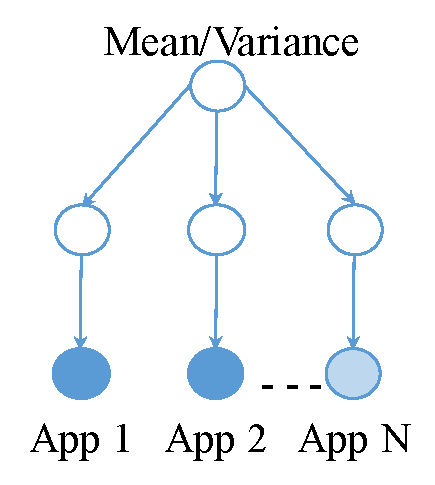
\includegraphics[width=.33\columnwidth]{figures/HBM.pdf}

    \label{fig:HBM}
  }
  \caption{ Comparison of online, offline, and hierarchical Bayesian
    models.  Arrows represent dependences, circles are random
    variables, white circles are hidden and must be learned, solid
    circles are fully observed data, and shaded circles are partially
    observed.}
\label{fig:learning-models}
\end{figure}


The HBM is a combination of the \emph{online} and \emph{offline}
approaches. The HBM incorporates both (1) observations of the current
application and (2) the previously observed applications to learn
correlations between different configurations.  The HBM's correlation
matrix captures these relations and scales with the number of
configurations, making the model non-parametric.  In practice, such a
non-parametric model is much more flexible; \eg{} it can learn a
linear relationship between frequency and performance for a
compute-bound application and that there is no relationship for a
memory-bound one.  Unlike the pure online approach, in the HBM all
models are conditionally dependent on a hidden mean and co-variance
matrix.  Rather than over-generalizing (like the offline model) or
over-specifying (like the online model) the HBM implicitly uses a pool
of similar applications to produce new models. Additionally, the HBM's
accuracy increases as more applications are observed because more
types of behavior are represented in the pool of prior knowledge.  Of
course, the HBM's computational cost -- which is linear in the number
of applications -- also increases with increasing applications, but
this is why we offload the learning to a remote server.

\subsection{The Lightweight Control System}

Control theory provides a discipline for tuning system parameters to
ensure that a system meets the desired goals in a dynamic environment.
We use a controller to adjust system resource usage to see that the
performance goals (corresponding to a quality-of-service or real-time
constraint) are met over time.  The difficulty is that classical
control formulations integrate the application-dependent relationship
between performance and the controlled resource directly in the
control formulation. This makes the control models too specific to a
particular class of applications.  Thus, we face the problem of
implementing a general control system that is applicable to a number
of applications, and where the models relating resources to
performance are not known ahead of time, but are provided by the HBM
at runtime.

\SYSTEM{} addresses this problem using the classic computer science
approach of adding a layer of indirection, as illustrated in
\figref{fig:framework:lcs}.  Instead of directly controlling resources
using an application-dependent model, \SYSTEM{} controls
\emph{speedup} and a separate module uses the learned models to
optimize energy while respecting this speedup constraint.  Similar
models have been used to build generalized controllers where users supply the models \cite{ControlWare,POET}.  Our
goal is to eliminate this user burden and have a remote HBM supply the
model\PUNT{, which are not just more accurate but become more
  intelligent with time as it acquires more data}.

\begin{figure}
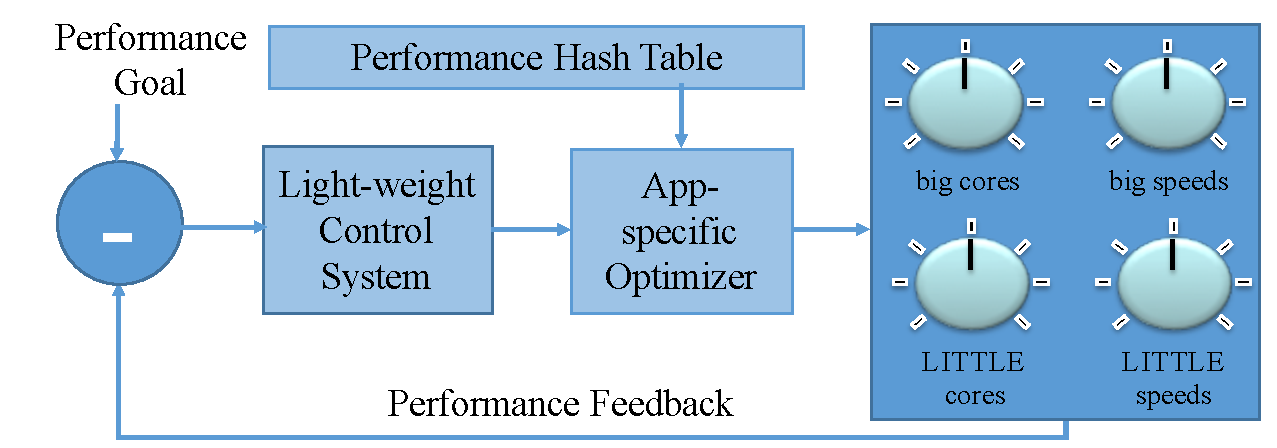
\includegraphics[width=\columnwidth]{figures/LCS.pdf}
\caption{Light-weight control system (LCS) }
  \label{fig:framework:lcs}
\end{figure}


\subsubsection{Controlling Speedup}
We write a simple difference model relating speedup to performance:
\begin{equation}
  perf(t) = m \cdot speedup(t-1) + \delta \label{eqn:speedup}
\end{equation}
where $m$ is the \emph{max speed} of the application, here defined as
the speed when all resources are available.  While $m$ is application
specific, it is easy to measure online, by simply allocating all
resources. Such a configuration should not violate any performance
constraints (although it is unlikely to be energy efficient) so it is
safe to take this measurement without risk of violating performance
constraints.

With this model, the control law is simply:
\begin{eqnarray}
  error(t) &=& goal - perf(t) \label{eqn:speedup-error} \\
  speedup(t) &=& speedup(t-1) - \frac{error(t)}{m}
  \label{eqn:speedup-control}
\end{eqnarray}
which states that the speedup to apply at time $t$ is a function of
the previous speedup, the error at time $t$ and the max speed $m$.
This is a very simple \emph{deadbeat} controller that provides all the
standard control theoretic formal guarantees \cite{Hellerstein2004a}.
Using the above definition of max speed, most speedups will be less
than one.  In addition to making max speed easier to measure, this
definition bounds the HBM's output, making for more robust learning.

\subsubsection{Optimizing Speedup}
\SYSTEM{} must turn the speedup produced by \eqnref{speedup-control}
into a resource allocation.  The primary challenge here is that since
the system resources are discrete, the HBM produces a non-linear
function mapping the resource allocations into speedup and powerup,
while \eqnref{speedup-control} is a continuous linear function.
\SYSTEM{} bridges this divide by assigning time to resource
allocations such that the average speedup over a control interval is
that produced by \eqnref{speedup-control}.

We call an assignment of time to resources a \emph{schedule}. We call
a combination of settings for each resource a \emph{configuration}.
For example, using two big cores at 1.5 \GHz and putting all the
little cores to sleep is one configuration.  There are typically many
schedules that meet a required speedup.  To extend battery life,
\SYSTEM{} finds a minimal energy schedule. Given a time interval $T$,
a workload $W$ to complete in that interval, and a set of $C$
configurations, we formalize this problem as:
\begin{eqnarray}
  \minimize_{\tau \in \mathbb{R}^C} && \sum_{c=0}^{C-1} \tau_c \cdot p_c \label{eqn:power} \\
  \text{such that} %&& \nonumber\\
  && \sum_{c=0}^{C-1} \tau_c \cdot s_c \cdot b =  W \label{eqn:work} \\
  && \sum_{c=0}^{C-1} \tau_c =  T \label{eqn:deadline} \\
  && 0 \le \tau_c \le T, \qquad \forall c \in \{0,\ldots,C-1\} \label{eqn:time}
\end{eqnarray}
where $p_c$ and $s_c$ are the estimated powerup and speedup of
configuration $c$ and $\tau_c$ is the amount of time to spend in
configuration $c$.  \eqnref{power} simply states that the objective is
to minimize energy (power times time).  \eqnref{work} states that the
work must be done, while \eqnref{deadline} requires the work to be
done on time.  \eqnref{time} simply avoids negative time.


\subsection{The Performance Hash Table}
While most linear programming problems would be inefficient to solve
repeatedly on a mobile device, the one in \eqnrref{power}{time} has a
constant time ($O(1)$ solution.  Kim et al. analyzed solutions to the
problem of minimizing energy while meeting a performance constraint
\cite{kim-cpsna}.  They observed that there must be an optimal
solution with the following properties:
\begin{itemize}
\item At most two of $\tau_c$ are non-zero, meaning that at most two
  resource configurations will be used in any time interval.  This
  property both drastically limits the search space and puts a limit
  on the overhead of switching configurations, since it is never
  profitable to switch more than twice in an interval.
\item If one plots the configurations in the power and performance
  tradeoff space (so that performance is on the x-axis and power is on
  the y-axis) the two configurations with non-zero $\tau_c$ lie on the
  lower convex hull of the power performance tradeoff space.
\end{itemize}
We use these two facts to construct a constant time algorithm for
finding the optimal solution to \eqnrref{power}{time} online.  The
intuition behind our solution is illustrated in the upper half of
\figref{fig:pht}.  This figure shows a hypothetical example of the power
and performance tradeoffs the HBM might learn for some application and
device.  Each point represents a configuration and each configuration
is charted with normalized performance on the x-axis and normalized
power on the y-axis.  For any feasible performance requirement, there
is a minimal energy schedule that uses no more than two of the
configurations on the lower convex hull as any points that lie above
the lower convex hull require more power for equivalent performance
\cite{kim-cpsna}.  Therefore, the HBM estimates the power and
performance of all configurations, then finds the lower convex hull,
and sends that to the LCS.  This lower convex hull is the interface
between the HBM and the LCS, and the key enabler of \SYSTEM{}'s
combination of learning and control.

% \begin{figure}
% 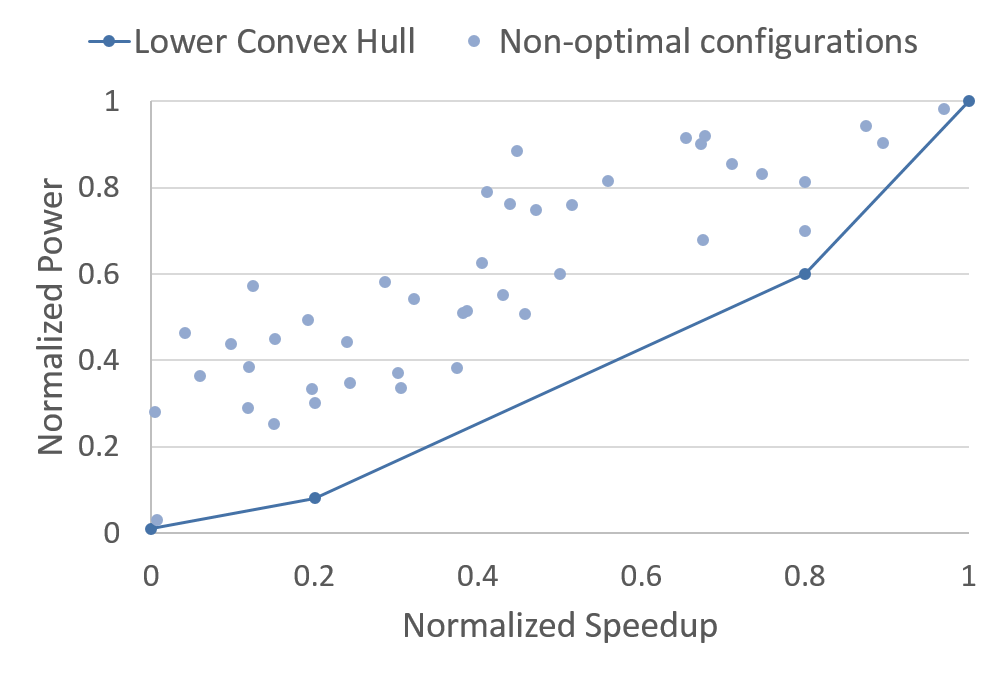
\includegraphics[width=\columnwidth]{figures/TradeoffExample.png}
% \caption{Example of plotting configurations in the power versus
%   performance space.}
%   \label{fig:convexhull}
% \end{figure}



\begin{figure}
  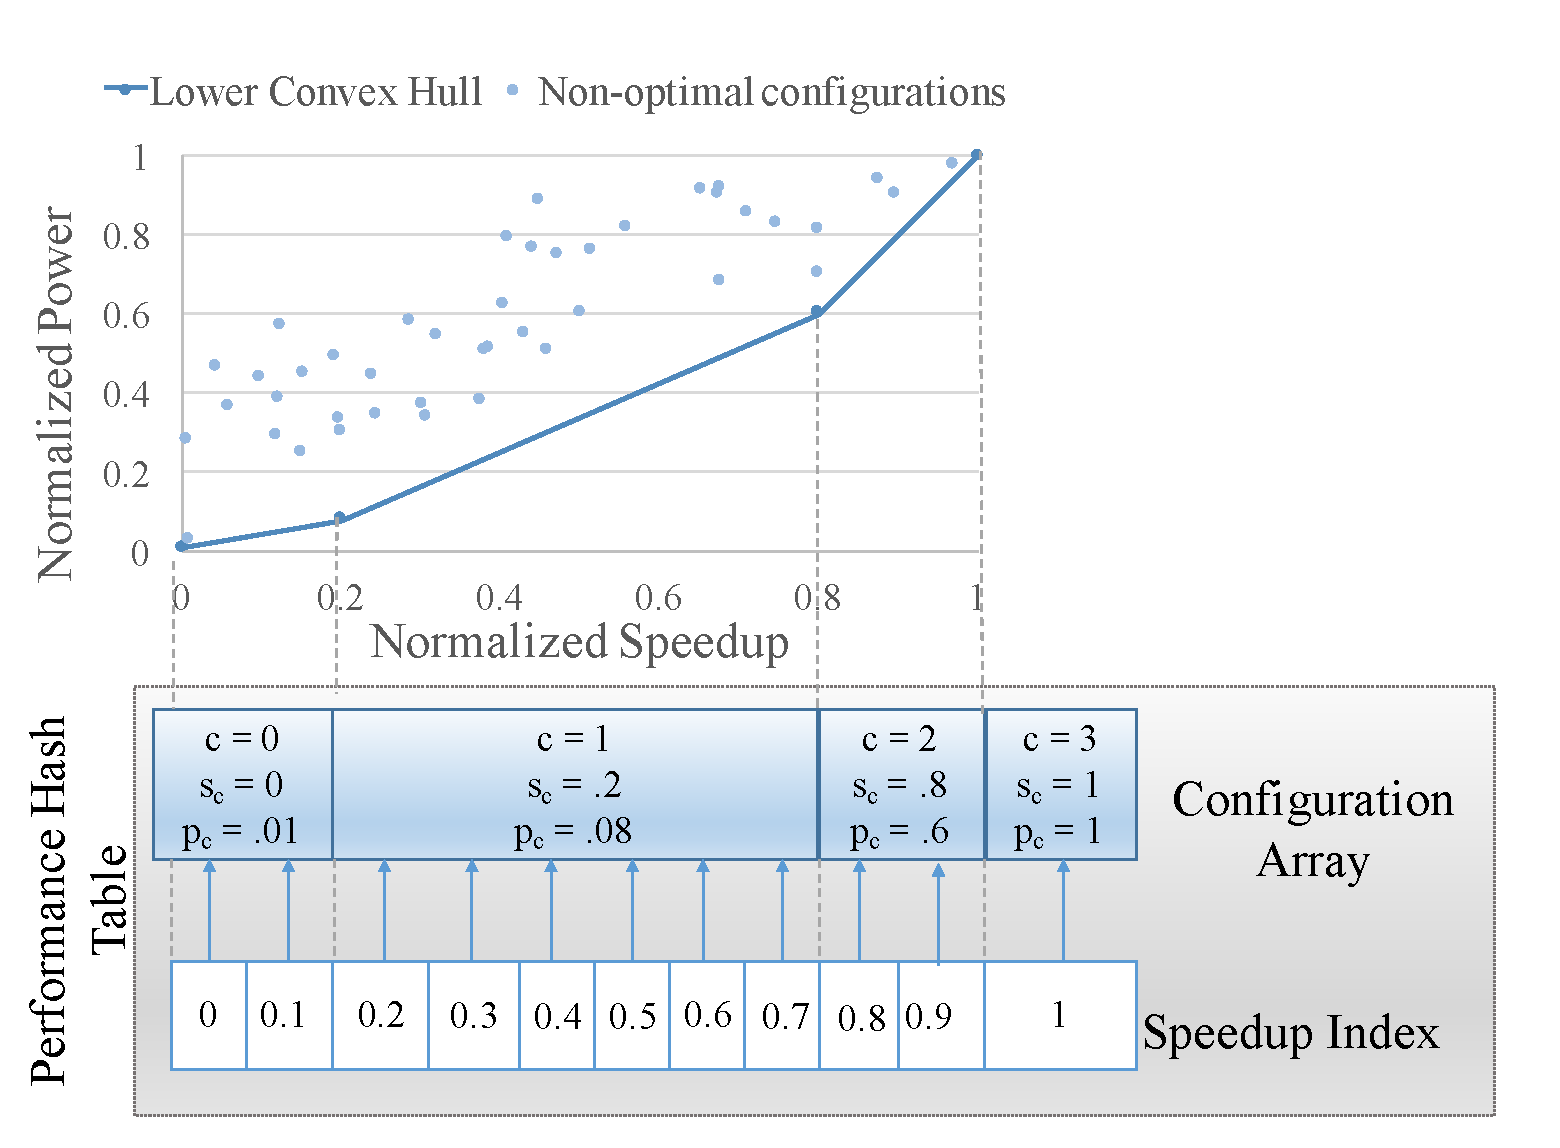
\includegraphics[width=\columnwidth]{figures/performance-hash-table.pdf}
  \caption{The Performance Hash Table and its relationship to the
    power/performance tradeoff space.  The HBM encodes the
    configuration as the lower convex hull of points in the
    performance/power tradeoff space and stores those in a table
    indexed by speedup.}
  \label{fig:pht}
\end{figure}

The HBM stores the lower convex hull in a \emph{performance hash
  table} (PHT).  The PHT and its relationship to the lower convex hull
is illustrated in \figref{fig:pht}.  It consists of two arrays, the
first is an array of pointers into the second array, which stores the
configurations on the lower convex hull sorted by speedup.  Recall
that speedups are computed relative to the maximum speed.  We
therefore know the largest speedup is 1, so we need only concern
ourselves with speedups less than 1.  The first table of pointers has
a \emph{resolution} indicating how many decimal points of precision it
captures.  The example in \figref{fig:pht} has a resolution of $0.1$.
Each pointer in the bottom table points to the configuration in the
second array that has the largest speedup less than or equal to the
index.

To use the table, the optimizer receives a speedup $s(t)$ from the
controller.  It needs to convert this into two configurations referred
to as $hi$ and $lo$.  To find the $hi$ configuration, the optimizer
clamps the desired speedup to the largest index lower than $s(t)$ and
then walks forward until it finds the first configuration with a
speedup higher than $s(t)$.  To find the $lo$ configuration, the
optimizer clamps the desired speedup to the smallest index higher than
$s(t)$ and then walks backwards until it finds the configuration with
the largest speedup less than $s(t)$.

\PUNT{
For example, consider the PHT in \figref{fig:pht} and an optimizer trying
to meet a speedup $s(t) = .65$.  To find $hi$, the optimizer indexes
at .6 and walks up to find $c=2$ with $s_c=.8$, setting $hi = 2$.  To
find $lo$, the optimizer indexes the table at .7 and walks backward to
find $c=1$ with $s_c=.2$, setting $lo = 1$.
}

Finally, the optimizer sets $\tau_{hi}$ and $\tau_{lo}$ by solving the
following set of equations:
\begin{eqnarray}
  \tau &=& \tau_{hi} + \tau_{lo}    \label{eqn:s1} \\
  s(t) &=& s_{hi} \cdot \tau_{hi} + s_{lo} \cdot \tau_{lo} \label{eqn:s2} 
\end{eqnarray}
In these equations, $s(t)$ is the speedup requested by the optimizer
and $s_c$ are speedups estimated by the learner.

By solving \eqnsref{s1}{s2}, the optimizer has turned the controller's
requested speedup into a resource allocation schedule using the models
provided by the HBM.  Provided that the resolution is large enough to
get a good spread of configurations to indices, the optimizer will
index the configuration one entry (on average) from where it needs to
be.  Thus, the entire optimization process runs in constant time --
assuming that the learner is responsible for building the PHT once
before passing it on to the optimizer.  This efficiency comes at a
cost of memory usage, as many of the entries in the speedup index
table will point to redundant locations in the configuration array.
This tradeoff is reasonable in practice as the code that runs on the
mobile device must be fast or we risk wasting energy while trying to
save energy.  In practice, we recommend a table of size 100 which
provides a sufficient resolution and is not too wasteful of space.

\PUNT{
\subsection{Putting It All Together}
We briefly summarize our proposal for combining learning and control.
Our approach consists of a number of independent mobile devices each
running a lightweight controller.  Each device makes a small number of
local observations of an application it runs and sends those to the
server.  The server integrates those observations in its HBM to
produce customized models for each device.  These models are sent back
to the individual devices where they are used to meet performance
requirements with minimal energy by turning a speedup signal into an
optimal schedule of configurations.

\TODO{The control theoretic guarantees are still valid provided that
  the error in the learned speedup is not too great.  Is it worth
  analyzing those formal guarantees?}

}

%control slowdown

%map slowdown into configurations

% solve optimization problem

% slowdown table

